\documentclass[crop,tikz]{standalone}

\usetikzlibrary{decorations.markings}
\tikzset{>=latex}

\begin{document}
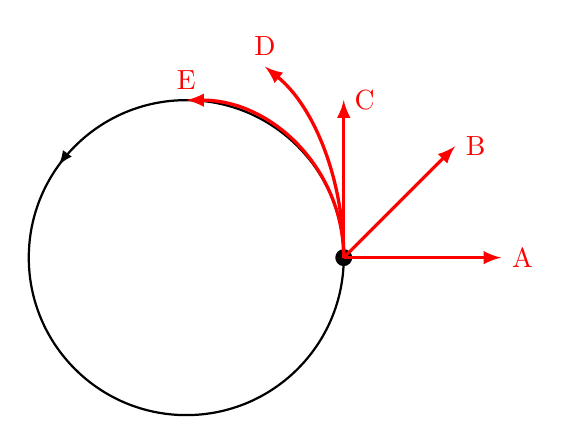
\begin{tikzpicture}[scale=2]
  \draw[
    decoration={markings, mark=at position 0.4 with {\arrow{>}}},
    postaction={decorate},
    thick
  ] (0,0) circle (1);
  \draw[fill] (0:1) circle (0.05);
  \draw[->,red,very thick] (0:1) -- +(0:1) node[right]{A};
  \draw[->,red,very thick] (0:1) -- +(45:1) node[right]{B};
  \draw[->,red,very thick] (0:1) -- +(90:1) node[right]{C};
  \draw[->,red,very thick] (0:1) arc (0:60:1 and 1.4) node[above]{D};
  \draw[->,red,very thick] (0:1) arc (0:90:1) node[above]{E};
\end{tikzpicture}
\end{document}
